\subsection{Trường vector}
\begin{frame}
    \frametitle{Trường vector}
    \begin{columns}
        \column{0.5\textwidth}
            \begin{figure}
                \centering
                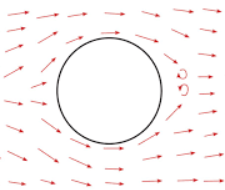
\includegraphics[width=4cm, height=3cm]{Content/Figure/streamline.png}
                \caption{Trường vận tốc của chất lưu}
            \end{figure}
            \[\mathbf{v}=\mathbf{v}(x,y)=\mathbf{v}(r,\theta)\]
        \column{0.5\textwidth}
            \begin{figure}
                \centering
                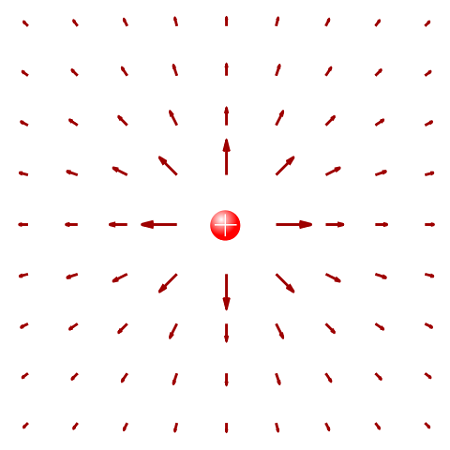
\includegraphics[width=4cm, height=3cm]{Content/Figure/electric_charge.png}
                \caption{Trường tĩnh điện của điện tích điểm}
            \end{figure}
            \[\mathbf{E}=\mathbf{E}(x,y,z)=\mathbf{E}(r)\]
    \end{columns}
\end{frame}
\subsection{Tính xoáy của trường}
\begin{frame}
    \frametitle{Trường (lực) thế}
    \begin{enumerate}
        \item Giá trị của tích phân đường (công) chỉ phụ thuộc vào điểm đầu và điểm cuối: \[-\int_{\mathbf{r}_1}^{\mathbf{r}_2}\mathbf{F}\cdot\text{d}\mathbf{l}=V(\mathbf{r}_1)-V(\mathbf{r}_2).\]
        \item Lưu số trên một đường cong kín là bằng không: \[\oint_{\mathcal{C}}\mathbf{F}\cdot\text{d}\mathbf{l}=0.\]
        \item Trường lực thế có thể biểu diễn dưới dạng gradient của một hàm vô hướng: \[\mathbf{F}=-\nabla V.\]
    \end{enumerate}
    \vspace{-5pt}

    Ví dụ về các lực thế: lực hấp dẫn, lực đàn hồi, \dots
\end{frame}
\begin{frame}
    \frametitle{Quan hệ giữa các tính chất của trường thế}
    \begin{columns}
        \begin{column}{0.5\textwidth}
            \scriptsize
            Từ tính chất thứ nhất,
            \[-\mathbf{F}\cdot\text{d}\mathbf{l}=\text{d}V.\]
            Do đó,
            \[-(F_x \text{d}x +F_y \text{d}y +F_z \text{d}z)=\partial_x V\text{d}x +\partial_y V\text{d}y +\partial_z V\text{d}z.\]
            Đồng nhất hai vế, 
            \[\mathbf{F}=-\nabla V.\]
        \end{column}
        \begin{column}{0.5\textwidth}
            \scriptsize
            Từ tính chất thứ hai (xét trên mặt phẳng \(xy\)),
            \begin{figure}
                \centering
                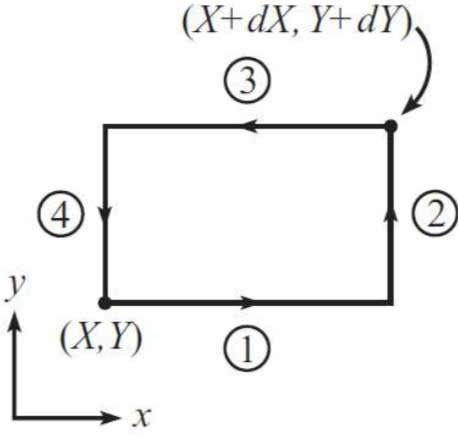
\includegraphics[width=3.5cm, height=3cm]{Content/Figure/Curl.jpg}
            \end{figure}
            \[\oint \mathbf{F}\cdot \text{d}\mathbf{l}=\text{d}X\text{d}Y\left(\partial_x F_y -\partial_y F_x\right)=0.\]
            Tương tự cho các mặt phẳng khác,
            \vspace{-5pt}
            \begin{align*}
                &\text{d}Y\text{d}Z\left(\partial_y F_z -\partial_z F_y\right)=0.&\\
                &\text{d}X\text{d}Z\left(\partial_z F_x -\partial_x F_z\right)=0.&
            \end{align*}
        \end{column}
    \end{columns}
\end{frame}

\begin{frame}
    \frametitle{Curl và định lý Curl (Stokes)}
    \begin{columns}
        \begin{column}{0.5\textwidth}
            \scriptsize
            Curl của \(\mathbf{F}\) được định nghĩa là
            \[\nabla\times\mathbf{F}\equiv \det\left(\begin{bmatrix}
                \hat{x} & \hat{y} & \hat{z}\\
                \partial_x & \partial_y & \partial_z\\
                F_x & F_y & F_z
            \end{bmatrix}\right).\]
            Định lý Stokes tổng quát hoá cho mọi bề mặt:
            \begin{equation*}
                \int_{\mathcal{S}}(\nabla\times\mathbf{F})\cdot\text{d}\mathbf{a}=\oint_{\mathcal{C}}\mathbf{F}\cdot\text{d}\mathbf{l}.
            \end{equation*}
            Chú ý, \(\mathcal{C}\) là đường biên của bề mặt \(\mathcal{S}\). Số hạng ở vế phải được gọi là \emph{lưu số} của trường \(\mathbf{F}\) trên đường cong kín \(\mathcal{C}\).
        \end{column}
        \begin{column}{0.5\textwidth}
            \scriptsize
            Curl của một trường thế bằng không nên \(\mathbf{F}\) phải có dạng \(-\nabla V\) vì
            \[\nabla\times(\nabla V)=0 \quad\forall V.\]
            Cụ thể,
            \begin{align*}
                \partial_{xy}V=&\partial_{yx}V,\\
                \partial_{yz}V=&\partial_{zy}V,\\
                \partial_{zx}V=&\partial_{xz}V.   
            \end{align*}
            Tóm lại, điều kiện cần và đủ của một trường thế là \[\nabla\times \mathbf{F}=\mathbf{0}.\]
        \end{column}
    \end{columns}
\end{frame}
\begin{frame}
    \frametitle{Minh hoạ cho dòng chảy xoáy}
    \begin{columns}
        \begin{column}{0.5\textwidth}
            \begin{figure}
                \centering
                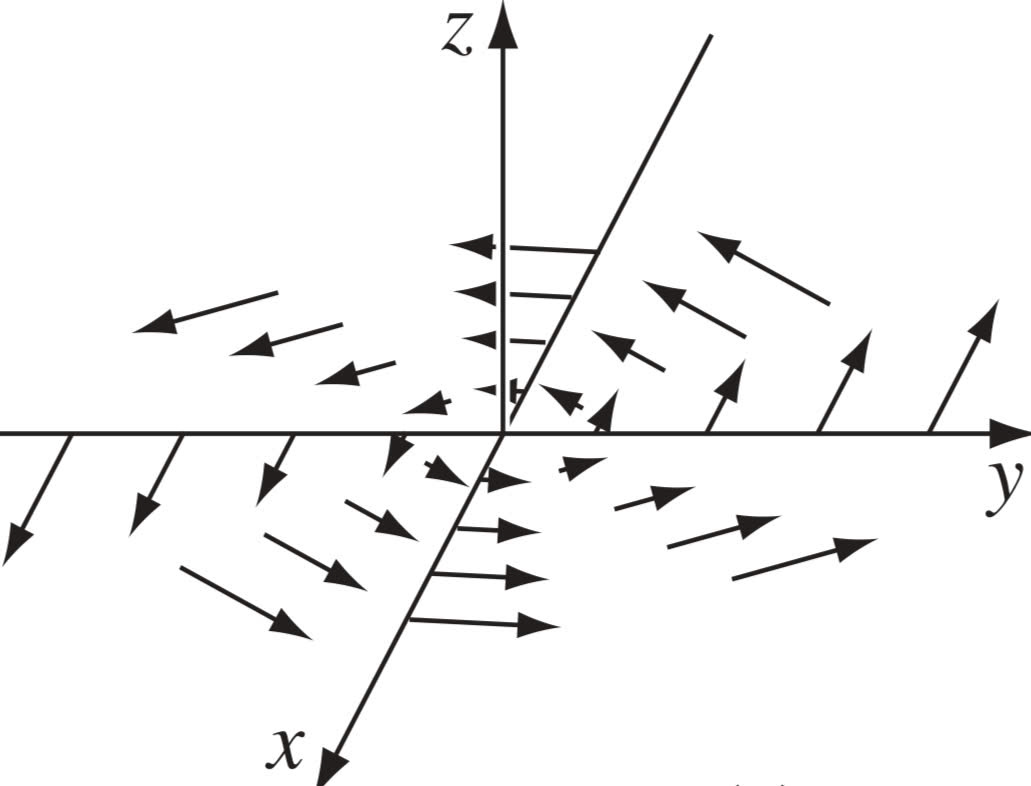
\includegraphics[width=4cm, height=3cm]{Content/Figure/illustration for curl.jpg}
            \end{figure}
            \[\mathbf{v}=-y\hat{x}+x\hat{y},\]
            \[\nabla\times\mathbf{v}=2\hat{z}.\]
        \end{column}
        \begin{column}{0.5\textwidth}
            \begin{figure}
                \centering
                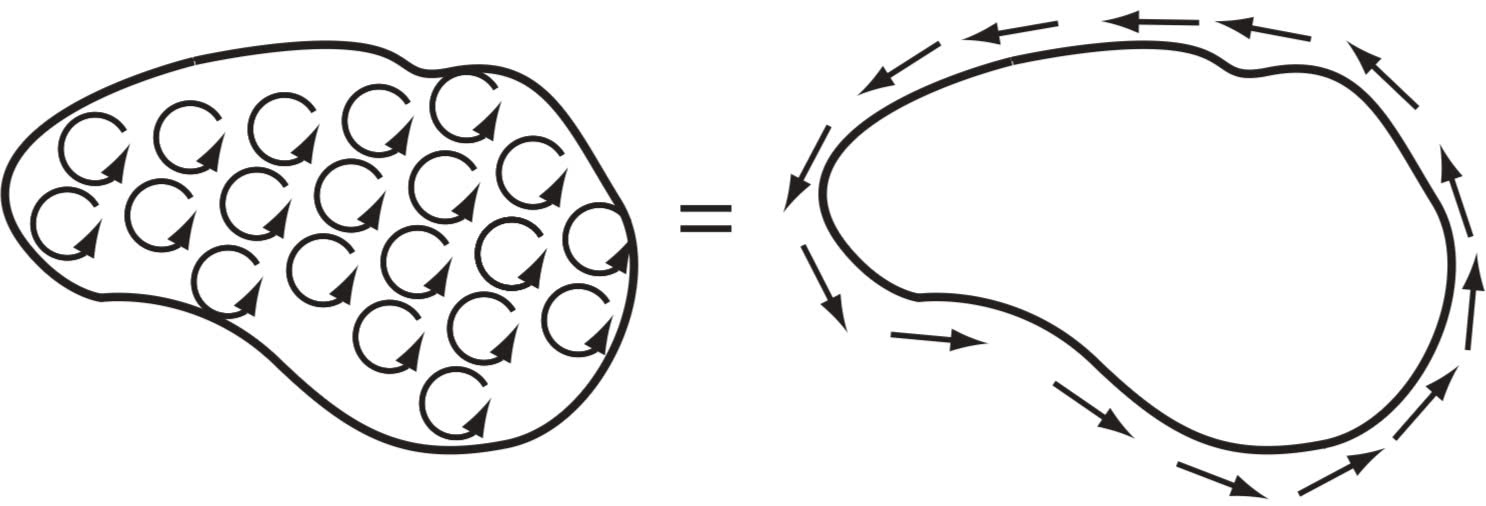
\includegraphics[width=4cm, height=2cm]{Content/Figure/illustration for Stoke.jpg}
                \caption{Định lý Stokes}
            \end{figure}
            \vspace{-8pt}

            \begin{figure}
                \centering
                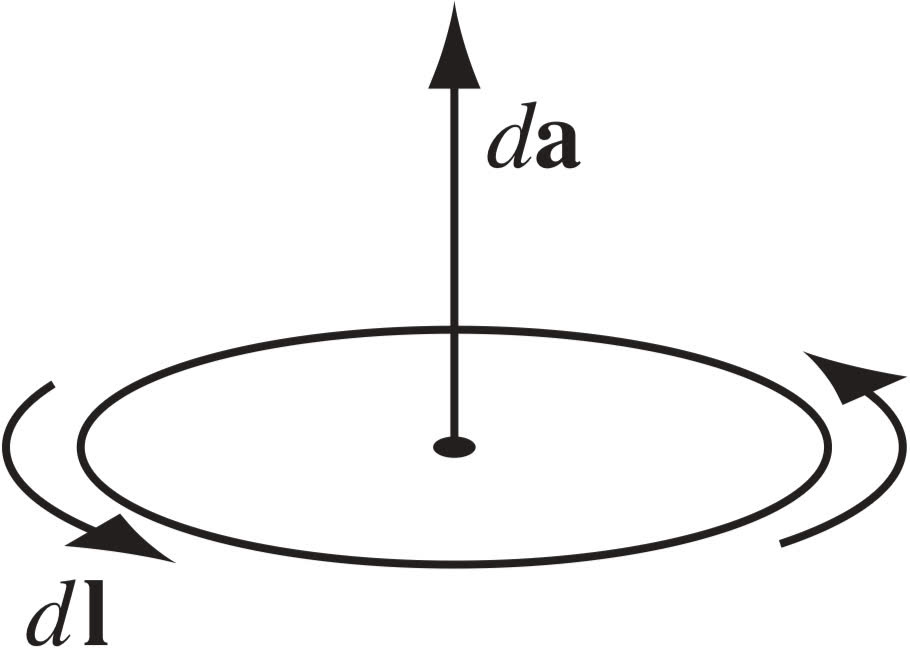
\includegraphics[width=2.5cm, height=2cm]{Content/Figure/direction_of_normal_vector.jpg}
                \caption{Chiều của vector pháp tuyến}
            \end{figure}
        \end{column}
    \end{columns}
\end{frame}
\subsection{Tính phân kỳ của trường}
\begin{frame}
    \frametitle{Thông lượng chất lỏng}
    \begin{figure}
        \centering
        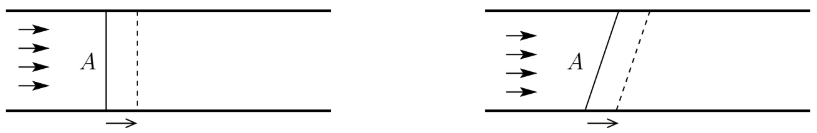
\includegraphics[width=14cm, height=3cm]{Content/Figure/flux of water.png}
    \end{figure}
    \[\text{Lượng nước đi qua tiết diện~}=\mathbf{v}\cdot\hat{n}A\Delta t.\]
    \[\text{Nếu tiết diện gấp khúc: }\sum_{i}^{n}\mathbf{v}\cdot \hat{n}_i A_i \Delta t.\]
    \vspace{-9pt}
    \[\text{Nếu tiết diện là một mặt cong liên tục: } \lim_{n\to\infty}\sum_{i}^{n}\mathbf{v}\cdot\hat{n}_i A_i \Delta t.\]
\end{frame}
\begin{frame}
    \frametitle{Tích phân mặt và thông lượng}
    \begin{figure}
        \centering
        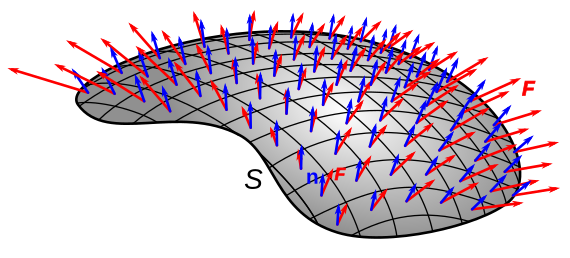
\includegraphics[width=8cm, height=4cm]{Content/Figure/curve_surface.png}
    \end{figure}
    \[\phi=\int_{\mathcal{S}}\mathbf{F}\cdot\text{d}\mathbf{a}.\]
    \(\phi\) được gọi là \emph{thông lượng} của trường \(\mathbf{F}\) qua bề mặt \(\mathcal{S}\).
\end{frame}
\begin{frame}
    \frametitle{Div và định lý Divergence (Gauss)}
    \begin{columns}
        \begin{column}{0.6\textwidth}
            \begin{figure}
                \centering
                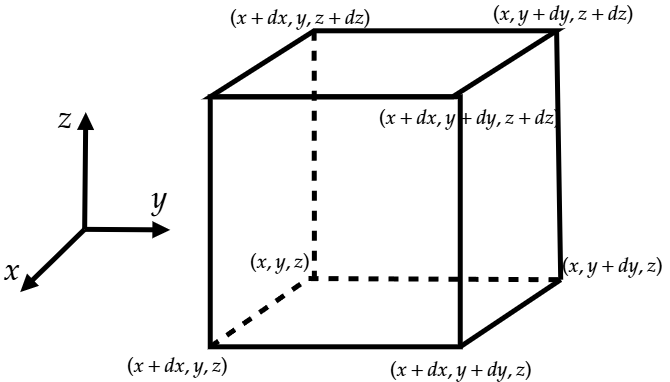
\includegraphics[width=8cm, height=5cm]{Content/Figure/infinitesimal_cube.png}
            \end{figure}
        \end{column}
        \begin{column}{0.4\textwidth}
            \scriptsize
            \begin{align*}
                \delta\phi=& (F_{x}(x+dx)-F_{x}(x))dydz \\
                          +& (F_{y}(y+dy)-F_{y}(y))dxdz \\ 
                          +& (F_{z}(z+dz)-F_{z}(z))dxdy\\
                          =& (\partial_x F_x +\partial_y F_y +\partial_z F_z)dxdydz.
            \end{align*}
            Với \(\nabla\cdot\mathbf{F}\equiv \partial_x F_x +\partial_y F_y +\partial_z F_z ,\)
            \[\delta\phi=\nabla\cdot \mathbf{F}\text{d}\tau.\]
            Định lý Divergence phát biểu rằng
            \begin{align*}
                \oint_{\mathcal{S}}\mathbf{F}\cdot \text{d}\mathbf{a}=\int_{\mathcal{V}}\nabla\cdot\mathbf{F}\text{d}\tau.
            \end{align*}
            
        \end{column}
    \end{columns}
\end{frame}
\begin{frame}
    \frametitle{Nguồn và giếng, phương trình liên tục}
    \begin{figure}
        \centering
        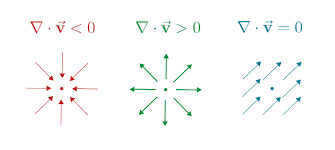
\includegraphics[width=6cm, height=3cm]{Content/Figure/sourrce_fluid.png}
    \end{figure}
    \[\oint_{\mathcal{S}}\mathbf{j}\cdot\text{d}\mathbf{a}+\frac{\partial }{\partial t}\int_{\mathcal{V}}\rho \text{d}\tau =0.\]
    \[\nabla\cdot\mathbf{j}=-\frac{\partial \rho}{\partial t}.\]
\end{frame}
\begin{frame}
    \frametitle{Hình ảnh ví dụ cho một trường vector với các xoáy, nguồn, và giếng}
    \begin{figure}
        \centering
        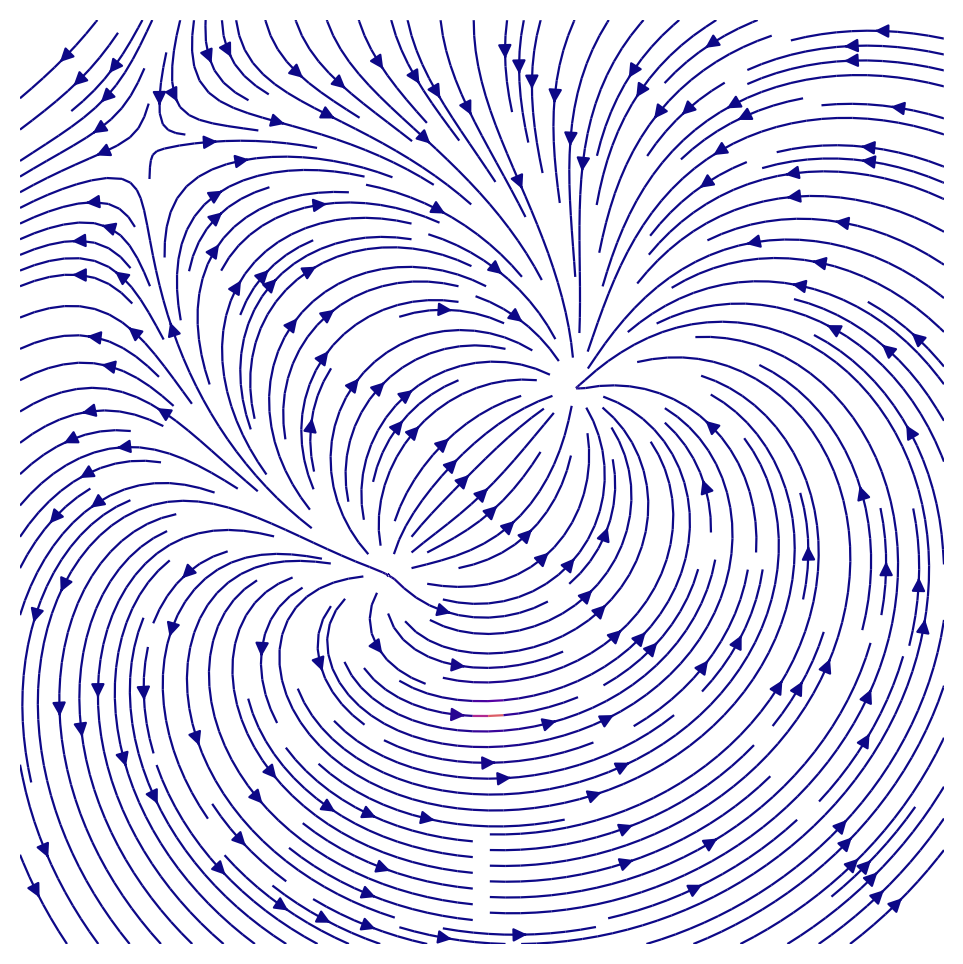
\includegraphics[width=9cm, height=6cm]{Content/Figure/vector_field_expressed.jpg}
    \end{figure}
\end{frame}
\begin{frame}
    \frametitle{Các đạo hàm}
    \begin{enumerate}
        \item \(\nabla\times(\nabla V)=0\) với mọi hàm vô hướng \(V\).
        \item \(\nabla\cdot(\nabla\times \mathbf{F})=0\) với mọi hàm vector \(\mathbf{F}\).
        \item \(\nabla\times(\nabla\times \mathbf{F})=\nabla(\nabla\cdot \mathbf{F})-\nabla^2 \mathbf{F}\), với \(\nabla^2\) là toán tử Laplace, được định nghĩa 
        \[\nabla^2 \equiv \partial^{2}_x +\partial^{2}_{y}+\partial^{2}_{z}.\]
    \end{enumerate}
    Ta cũng có thể viết \[\nabla^2 \mathbf{F}=(\nabla\cdot\nabla)\mathbf{F}.\]
    \scriptsize
    Ngoài ra, \[(\mathbf{u}\cdot\nabla)\mathbf{F}\] biểu thị xấp xỉ tuyến tính cho "vi phân" của \(\mathbf{F}\):
    \vspace{-5pt}
     \[\mathbf{F}(\mathbf{r}+\mathbf{u})-\mathbf{F}(\mathbf{r})\approx (\mathbf{u}\cdot\nabla)\mathbf{F}.\]
\end{frame}
\subsection{Một số ứng dụng}
\begin{frame}
    \frametitle{Áp suất-phương trình cân bằng thuỷ tĩnh}
    Một hệ quả quan trọng của định lý Divergence, với một vô hướng \(T\), là 
    \[\int_{\mathcal{V}}(\nabla T)\text{d}\tau =\oint_{\mathcal{S}}T\text{d}\mathbf{a}.\]
    Với áp suất \(p\) trong chất lỏng, phương trình thu được là 
    \[\int_{\mathcal{V}}(\nabla p)\text{d}\tau =\oint_{\mathcal{S}}p\text{d}\mathbf{a}.\]
    Như vậy, \[-\nabla p +\mathbf{f}_V =\mathbf{0},\] với \(\mathbf{f}_V\) là lực thể tích.
    Trong trường trường hợp của trọng trường,
    \vspace{-5pt}
    \[\nabla p=\rho \mathbf{g}.\]
\end{frame}
\begin{frame}
    \frametitle{Lực hấp dẫn của một khối/vỏ cầu đồng nhất}
    \begin{columns}
        \begin{column}{0.5\textwidth}
            \vspace{-5pt}

             \begin{figure}
        \centering
        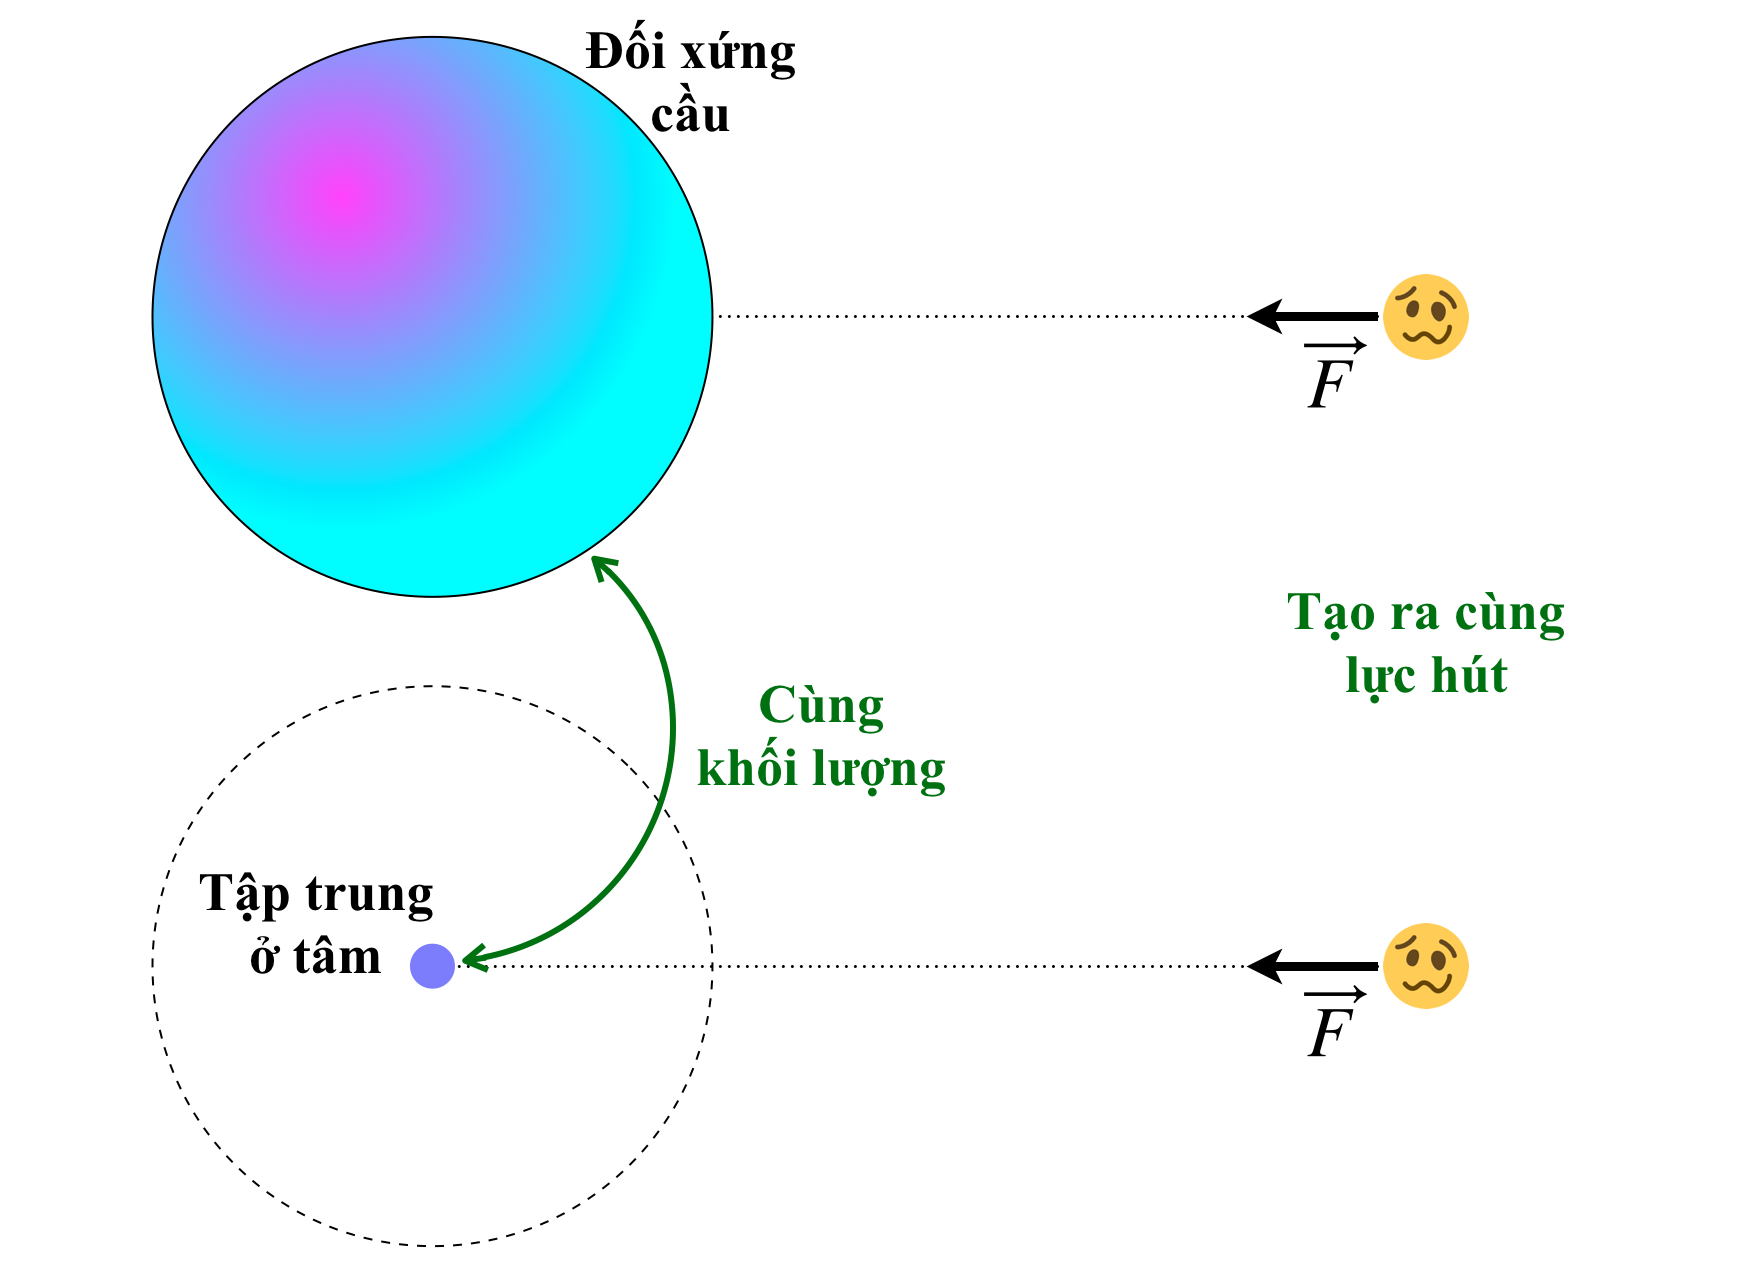
\includegraphics[width=7cm, height=5cm]{Content/Figure/gravity.png}
    \end{figure}
        \end{column}
        \begin{column}{0.5\textwidth}
            \scriptsize
            \[\nabla\cdot\mathbf{F}=\frac{1}{r^2}\partial_r(r^2 F_r)=-4\pi G \rho.\]
           \[\implies (\mathbf{F}\cdot\hat{r})\oint_{\mathcal{S}}da =-4\pi G \rho\times \frac{4\pi}{3}R^3.\]
           \[\implies F_r =-\frac{4\pi G\rho}{3} \frac{R^3}{r^2}.\]
           \[\implies F_r =-\frac{GM}{r^2}\]
            Với \(M=\frac{4\pi R^3}{3}\rho\). Ở đây ta đã đặt \(m=1 kg\).
   \end{column}
    \end{columns}
\end{frame}
\begin{frame}
    \frametitle{Bốn phương trình Maxwell trong chân không}
    \begin{enumerate}
        \item  Định lý Gauss \[\nabla\cdot\mathbf{E}=\varepsilon_{0}^{-1}\rho .\]
        \item  Định lý về sự không tồn tại của đơn cực từ \[\nabla\cdot\mathbf{B}=0.\]
        \item  Định luật Faraday\[\nabla\times\mathbf{E}=-\partial_t \mathbf{B}.\]
        \item Định lý Ampere-Maxwell \[\nabla\times\mathbf{B}=\mu_0 \mathbf{J}+\mu_0\epsilon_0 \partial_t \mathbf{E}.\] 
    \end{enumerate}
\end{frame}
\begin{frame}
    \frametitle{Điện trường của điện tích điểm }
    \begin{columns}
        \begin{column}{0.3\textwidth}
            \begin{figure}
                \centering
                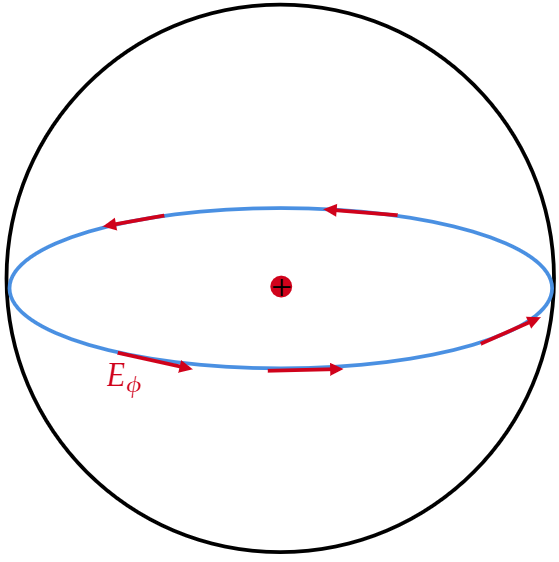
\includegraphics[width=3.5cm, height=3.5cm]{Content/Figure/azimuthal_field.png}
            \end{figure}
            \[E_{\phi}2\pi r =0.\] \[\implies E_{\phi}=0.\]
        \end{column}
        \begin{column}{0.3\textwidth}
            \begin{figure}
                \centering
                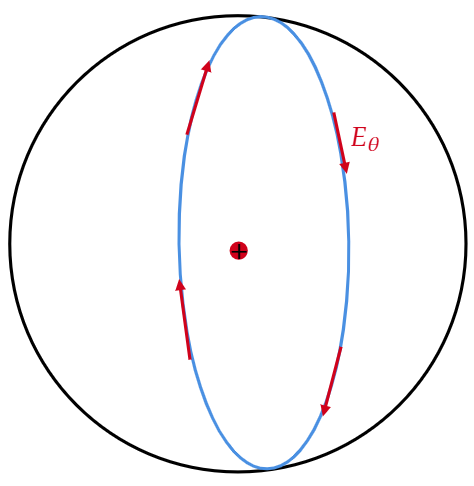
\includegraphics[width=3.5cm, height=3.5cm]{Content/Figure/theta_field.png}
            \end{figure}
            \[E_{\theta}2\pi r =0.\] \[\implies E_{\theta}=0.\]
        \end{column}
        \begin{column}{0.3\textwidth}
            \scriptsize
            Trong tĩnh điện, \(\nabla\times\mathbf{E}=\mathbf{0}\). Thành thử, \[\oint_{\mathcal{C}}\mathbf{E}\cdot\text{d}\mathbf{l}=0.\implies \mathbf{E}=\mathbf{E}_r \hat{r}.\]
            Điều kiện biên:\vspace{-5pt} \[\lim_{r\to\infty}\mathbf{E}(r)\to\mathbf{0}.\]
            Định lý Gauss:\vspace{-5pt} \[\oint_{\mathcal{S}}\mathbf{E}\cdot\hat{r}~da =\varepsilon_{0}^{-1}q.\]
            Như vậy, \vspace{-5pt}\[\mathbf{E}=\frac{1}{4\pi\varepsilon_0}\frac{q}{r^2}\hat{r}.\]
        \end{column}
    \end{columns}
\end{frame}
